\section{Process discovery through Grammar Inference} \label{grammar}
One of the relevant to my research work was done by Cook \& Wolf in \cite{citeulike:328044}. Authors developed a \textit{``process discovery''} techniques aiming a discovery of process models from event streams. Authors did not really aim at the retrieval of a complete and correct model, but a retrieval of sub-models that express the most frequent patterns in the event stream. They designed a framework which collects a software process data from ongoing process or from the history logs and generates a set of recurring patterns of behavior characterizing observed process. Under this work they augmented two methods of \textit{grammar inference} from previous work: statistical (neural network based \textit{RNet}) and purely algorithmic (\textit{KTail}) as well as developed their own Markovian method (\textit{Markov}). 

The \textit{process discovery} by the authors opinion resembles the process of \textit{grammar inference}, which can be defined as the process of inferring a language grammar from the given set (sample) of sentences in this language. In the demonstrated approach, words of the language are atomic events of the dynamic process, whether sentences are describing the behavior of a process and built from such words. Consequently, the inferred grammar of that language is then the formal model of the process. Cook \& Wolf expressed such grammars as Finite State Machines (FSMs) and implemented a software tool and successfully employed it in an industrial case study.

\begin{figure}[tbp]
   \centering
   \includegraphics[height=70mm]{inference.eps}
   \caption{Process discovery through the grammar inference: panel a) a sample event stream (simple process involving three types of events: Edit, Review, and Checkin); and FNA results obtained by applying three methods of process discovery from Cook \& Wolf \cite{citeulike:328044}.}
   \label{fig:inference}
\end{figure}

The first method, neural network based grammar inference method RNet, adopted by authors defines a recurrent neural network architecture which is trained by the sequences of events and after training able to characterize a current system state by looking on the past behavior. Once the neural net is trained, authors extract the FSM by presenting different strings to the net and extracting the hidden neurons activity through observations: by the nature of Neural Net, the closely related activation patterns clustered into the same state; by noting the current pattern, the input token, and the next activation pattern, transitions are recorded and compiled into inferred FSM.

The second method adopted, a purely algorithmic KTail method, taken from Biermann \& Feldman \cite{citeulike:5120603}. The idea is that a current state is defined by what future behaviors can occur from it. The \textit{future} here is defined as the set of next $k$ tokens. By looking at a window of successor events KTail algorithm is building the equivalence classes that compose the process model. Authors extensively modified the original KTail algorithm improving the folding in the mined model making it robust to noise.

The Markov based method developed by authors is resting on the algorithmic and statical approaches. It takes in account past and future system behavior in order to guess the current system state. Assuming that a finite number of states can defined the process, and that the probability of the next state is based only on the current state (Markov property) authors build a $n^{th}$-order Markov model using the first and second order probabilities. Once built, the transition probability table corresponding to the Markov model is converted into FSM which further reduced basing on the user specified cut-off threshold for probabilities.

Authors implemented all discussed algorithms in a software tool called DaGama as a plugin for larger software system called Balboa \cite{citeulike:5120757}. By the benchmarking, Cook \& Wolf proved the Markov algorithm superiority to the other two algorithms. RNet was found the worst of the three algorithms. 

Overall, while having some issues with the complexity of produced output and noise handling, authors proved applicability of implemented algorithms to the real-world process data by demonstrating an abstraction of the actual process executions and capturing important properties of the process behavior. Major backdraw of the approach, as stated by authors, lies in the inability of the FSMs to model concurrency of processes whether the software development process is usually performed by the many agents simultaneously. This limitation was addressed later by Cook et al \cite{citeulike:5128143}.
